\documentclass[a4paper]{article}

\usepackage{geometry}
\usepackage{graphicx}
\usepackage{array}

\newcolumntype{L}{>{\centering\arraybackslash}p{3.3cm}}
\newcolumntype{D}{>{\centering\arraybackslash}p{5cm}}
\newcolumntype{I}{>{\centering\arraybackslash}p{3cm}}

\title{LightBox $lightBoxNumber - $pmSN}
\author{}

\begin{document}
\maketitle


\section{PM infos}

\def\imagetop#1{\vtop{\null\hbox{#1}}}
\begin{tabular}{lr}
% \begin{tabular}{|L|L|L|L|}
% 	\hline
% 	Serial Number		& Position in LightBox 		& Cathode Luminous Sens. 	& Anode Luminous Sens.\\
% 						&							& \$\mu A/lm\$				& \$A/lm\$ \\
% 	\hline
% 	HB9050 				& 12						& 74.7						& 89.6 \\
% 	\hline
% 	Anode Dark Current 	& Cathode Blue Sens. Index 	& Gain Anode/Cathode 		& \\
% 	nA					& 							&  							& \\
% 	\hline
% 	0.01 				& 9.44						& 1.20E+06					& \\
% 	\hline
% \end{tabular}
\begin{tabular}[t]{|D|I|}
	\hline
	Serial Number			& $pmSN \\
	\hline
	Position in LightBox 	& $pm.GeoPos \\
	\hline
	Cathode Luminous Sens. \newline\$\mu A/lm\$	& $pm.CatLum \\
	\hline
	Anode Luminous Sens. \newline\$A/lm\$	& $pm.AnLum \\
	\hline
	Anode Dark Current 	\newline\$nA\$	& $pm.DarkCurr \\
	\hline
	Cathode Blue Sens. Index 	& $pm.BlueSens \\
	\hline
	Gain Anode/Cathode 		& $pm.Gain \\
	\hline
\end{tabular}
&
\imagetop{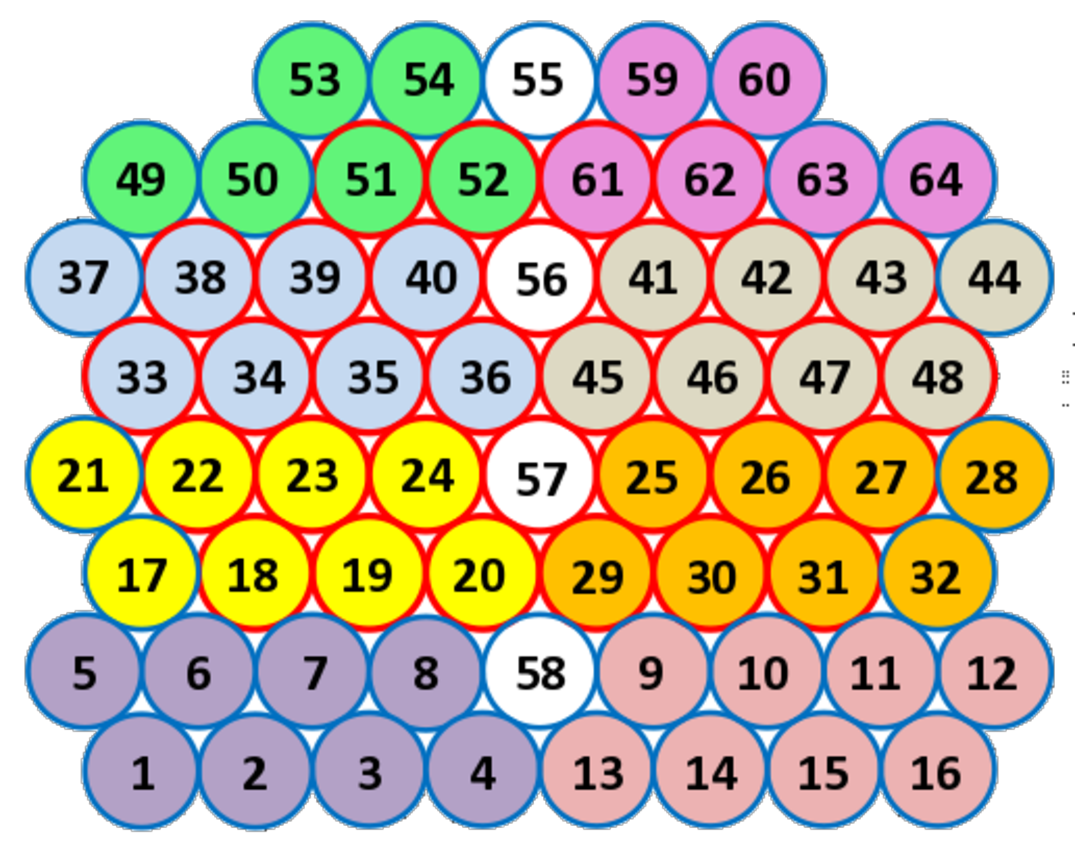
\includegraphics[scale=0.3]{lightBoxGeo.pdf}}\\

\end{tabular}
\section{Run results}

\end{document}